\documentclass[12in]{article}

\usepackage{xcolor}
\usepackage{natbib}
\usepackage{apalike}
\usepackage[colorlinks=true]{hyperref}
\usepackage{tikz}
\usepackage{caption}
\usepackage{subcaption}

\title{Application to the
\href{https://www.ukri.org/opportunity/bioinformatics-and-biological-resources-fund-24bbr/}{BBR24}
funding opportunity\\\vspace{.5in}Enabling the Next Generation of Naturalistic Long-Duration Neuroscience
Experimentation with Advanced Machine Learning}

\begin{document}

\tableofcontents

\pagebreak

\maketitle

\section{Summary}

\textcolor{red}{Word limit: 550}

\textcolor{red}{In plain English, provide a summary we can use to identify the
most suitable experts to assess your application.}

{\color{red}

Clearly describe your proposed work in terms of:

\begin{itemize}
\item context
\item the research the infrastructure, facility or resource will enable
\item aims and objectives
\item potential user communities, applications and benefits
\end{itemize}
}

\subsection{Context}

% add references
The use of large amounts of data in image and speech recognition and more
recently in large language models has generated breakthroughs in the
capabilities of machine learning models. Yet, most animal experiments in
Neuroscience still generate limited amounts of data, as animal behaviour is
heavily constrained and the duration of experiments is short.
%
Long-duration experiments, where animals can move freely in naturalistic
environments, combined with advanced machine learning methods, could reveal new
aspects of behaviour and brain function not evident in data generated in
simpler experiments.
%
At the Sainsbury Wellcome Centre (SWC) for Neural Circuits and Behaviour we are
performing long-duration and naturalistic foraging experiments.
%
Here we propose to create a resource to share openly online and offline machine
learning methods to process behavioural and neural data generated by these
experiments. Every method shared in this resource will be demonstrated with
data from the SWC foraging experiments.

\subsection{The research the infrastructure, facility or resource will enable}

Advanced machine learning software is essential to extract insights from the
data generated by naturalistic and long-duration experiments. Thus, the software
disseminated by our resource will be essential to extract insights from these
experiments and could generate valuable findings.

In addition, the evaluation of different models on our foraging datasets should
help researchers analysing long-duration and naturalistic experiments choose the
best models for their needs, accelerating their research.

Our resource could also motivate research and development on novel machine
learning methods for controlling and characterising long-duration and
naturalistic experiments, as our foraging datasets could act as a testbed for
methods comparison, and machine learning scientists may want to develop methods
to excel in this comparison.

\subsection{Aims and objectives}

The first aim of the proposed resource is to enable a new type of
long-duration and naturalistic animal experimentation, by sharing well-tested
machine learning methods for online and offline processing of data generated by
these experiments.

A second aim is to build a resource that is a reference where the best machine
learning methods to control and characterise long-duration naturalistic
experiments can be compared against each other on state-of-the-art foraging
datasets.

\subsection{Potential user communities, applications and benefits}

The following user communities could benefit from the proposed resource:

\begin{description}

    \item[research groups investigating data from long-duration naturalistic
        experiments] could use the distributed machine learning software to analyse their
        data and generate scientific discoveries.

    \item[business entities] using long-duration and/or naturalistic
        experiments could benefit from our distributed software and improve
        their processes. For example, pharmaceutical businesses are starting to
        use whole animal screening to test for side effects on drugs. They
        could use our distributed software to improve animal behavioural and
        neural monitoring.

    \item[machine learning methods developers] could contribute their methods
        to the resource, so that they are evaluated on our foraging data, and
        become known to users of our repository.

\end{description}



\pagebreak

\section{Core team}

{\color{red}

List the key members of your team and assign them roles from the following:

\begin{itemize}
	\item project lead (PL)
	\item project co-lead (UK) (PcL)
	\item researcher co-lead (RcL)
	\item specialist
	\item professional enabling staff
	\item research and innovation associate
	\item technician
	\item visiting researcher
\end{itemize}

Only list one individual as project lead.

A research technical professional or research software engineer can be listed
as a project lead or project co-lead, provided that:

\begin{itemize}

	\item their appointment is resourced from the central funds of their research
organisation at the time of application

	\item their level of responsibilities and duties is appropriate to a person with
substantial research experience

	\item their contract extends beyond the duration of the project

\end{itemize}

The researcher co-lead role has replaced the research co-investigator role
previously used in Je-S grant applications. They will be an individual who merits
appropriate recognition for making a substantial contribution to the formulation
and development of the application and will be closely involved with the project.

}


\begin{description}
    \item[project lead (PL)] Prof.~Tiago Branco
    \item[project co-lead (UK) (PcL)] Prof.~Maneesh Sahanai, Prof.~Thomas Mrsic-Flogel
    \item[researcher co-lead (RcL)] Dr.~Joaquin Rapela, Dr.~Goncalo Lopez,
        Dr.~Dario Campagner, Dr.~Adam Tyson
    \item[specialist] Dr.~Nicholas Guilbeault
    \item[research and innovation associate] Dr.~Lorenza Calcaterra
\end{description}


\pagebreak

\section{Application questions}

\subsection{Vision}

{\color{red}

Word limit: 1,700

What are you hoping to achieve with your proposed work?

What the assessors are looking for in your response

Explain how your proposed work:

\begin{itemize}

\item is of excellent quality and importance within or beyond the field(s) or area(s)

\item has the potential to advance current understanding, or generate new
knowledge, thinking or discovery within or beyond the field or area

\item is timely given current trends, context, and needs

\item impacts world-leading research, society, the economy, or the environment

\end{itemize}

Include the following in your statement:

\begin{itemize}

\item the uniqueness and expected added value of the proposed resource to the
UK bioscience research community and infrastructure landscape

\item how the resource relates to past and current resources in the subject area in
both the UK and abroad

\item full details of the resource and an overview of the associated objectives.
Details on how these objectives are delivered should be included in the
Approach section

\item a description of the types of research that will be enabled by the resource

\item consideration of the potential impact on the scientific community and other
possibly dependent resources if the resource did not exist

\item only if applicable, relevance of the proposed work to the plant health spotlight

\end{itemize}

In your vision, you should also clearly identify which of the following categories
your proposed resource falls under, and expand on the relevant points raised
below:

\begin{itemize}

\item establishment of a new and innovative resource that will be beneficial to a
broader BBSRC user base. Explain why a new resource is needed and what
unique and important features it will offer
\item maturation and subsequent maintenance of a project-based resource into a
community-based one. Briefly explain the background to the resource,
current usage, proposed changes and the benefits this will lead to for the
research community
\item further development or essential maintenance of an existing community
resource, with well-established access mechanisms. Explain current usage
and how this project will increase its relevance, quality and utility, for
example:

\begin{itemize}

\item by enabling the resource to support FAIR (findable, accessible,
interoperable, reusable) principles
\item by enabling new uses, for example metadata enrichment for machine
learning and AI approaches

\end{itemize}

\item association, or integration, of distinct resources. Explain current usage and
how the proposed plans will create an upgraded resource with a greater
value than the sum of the parts

\end{itemize}

References may be included within this section.

You may demonstrate elements of your responses in visual form if relevant.
Further details are provided in the Funding Service.
}

\subsubsection*{Conventional versus modern neuroscience experimentation}

Conventional system neuroscience experiments heavily constrain the behaviour of
their subjects in order to simplify behavioural and neural analysis.  However,
important aspects of brain function may not be expressed in these constrained
behaviours and these aspects may only manifest in naturalistic experimental
conditions.

% recent foraging experiments
% -> need of advanced machine learning methods to extract information from these experiments

Recent technological advances now allow to build complex naturalistic
experiments, while measuring a large number of experimental variables and
recording from a large number of neurons simultaneously. These advances
allow unrestrained subjects behaviour with precise monitoring of what happens in
the subjects' environment and brain.

Important examples of these experiments are naturalistic foraging experiments,
where freely moving subjects search for food in unrestrained environments.
Foraging studies are currently underway at major research centres around the
world (e.g., the Allen Institute for Brain Research, Janelia Farm, the Max
Plank Institute of Animal Behaviour).

A complication of naturalistic neuroscience experiments is extracting meaning
from the plethora of data that they generate \citep{juavinett22}. Machine
learning methods are specially helpful to address this problem. For example,
they can be used to extract subjects' internal states from behavioural
measurements, to extract low-dimensional latent variables from high-dimensional
neural recordings, and to relate the inferred subjects' internal state to the
neural latent variables.

The data generated by conventional system neuroscience experiments can be
understood by just plotting a few of its variables. However, interpreting the output
of naturalistic experiments is more difficult and machine learning methods
become essential for this.

\subsubsection*{Long-duration and naturalistic experiments at the SWC}
% at the SWC we are performing a new type of foraging experminets

At the SWC we are performing a novel type of naturalistic and long-duration
foraging experiments. Mice are housed in large circular arenas
(Figure~\ref{fig:arena}a)
equipped with a shelter, where animals can rest and drink, and with food patches,
where animals can get food pellets after moving a wheel for a fixed
configurable distance (Figure~\ref{fig:arena}b). Mice live in the arena for extended periods of time. We
monitor the behaviour of mice in detail with multiple high-resolution video
cameras, to monitor the positions of mice body parts, ultrasound audio cameras,
to monitor mice vocalisations, and a scale in the shelter, to regularly measure
mice weights. We record neural activity using Neuropixel probes with 5,000
channels, from which 384 channels can be selected for recording, and with
64-channel probes, equipped with an electrical stimulator and an optical
stimulator.
%
We running foraging experiments with one or multiple mice per arena.

\begin{figure}
    \begin{subfigure}{\textwidth}
        \centering
        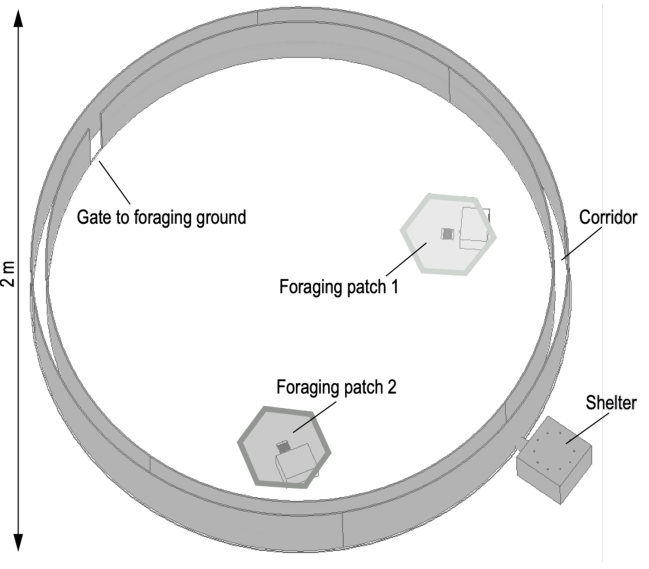
\includegraphics[width=4in]{figures/arena.png}
        \caption{}
    \end{subfigure}
    \par\bigskip
    \begin{subfigure}{\textwidth}
        \centering
        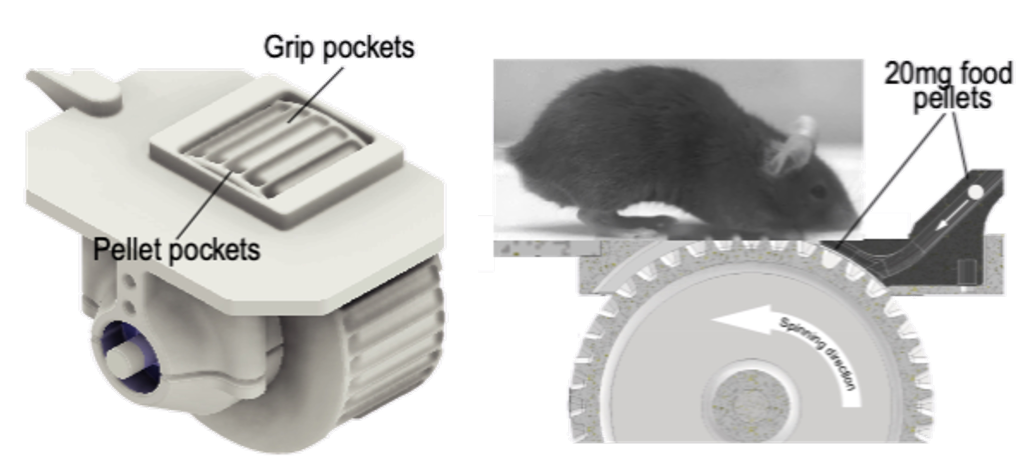
\includegraphics[width=4in]{figures/patch.png}
        \caption{}
    \end{subfigure}
    \caption{Foraging arena (a) and patch (b).}
    \label{fig:arena}
\end{figure}

A unique feature of our foraging experiments is their long duration. We have
already recorded behaviour and neural activity of mice continuously for 48 hours
and by the end of 2024 we aim at recording continuously for two weeks.

These long-duration experiments are allowing us to address foraging questions
that cannot be studied in shorter experiments. For example, scientifically
these experiments allow us to ask how do mice foraging patterns change across
days, and what are the neural mechanisms underlying these changes.
Statistically, the large amount of data recorded in the new experiments allows
us to estimate parameters of much more complex models than those that can be
fitted to data from conventional system neuroscience experiments.

% normative versus statistical characterization of foraging behavior
% The most common characterization of foraging experiments is a principled one,
% based on the marginal value theorem~\citep{charnov74}. It states that a subject
% will leave a patch when the reward rate of the patch falls below the average
% reward rate in the environment. Naturalistic and long-duration experiments
% allow us to attemp statistical characterizations of foraging experiments

% The naturalistic and long-duration experiments

\subsubsection*{Proposed resource}
% the proposed project

The initial SWC foraging project was core funded and the generated by it data
has been exclusively used by interal scientists. Here we propose to mature this
foraging project and create a resource to (1) share data from our long-duration
naturalistic foraging experiments, (2) share machine learning software
implementations of methods to simulate and analyse these data and (3) organise
foraging data simulations and analysis competitions
(Figure~\ref{fig:resource}).

\begin{figure}
    \begin{center}
        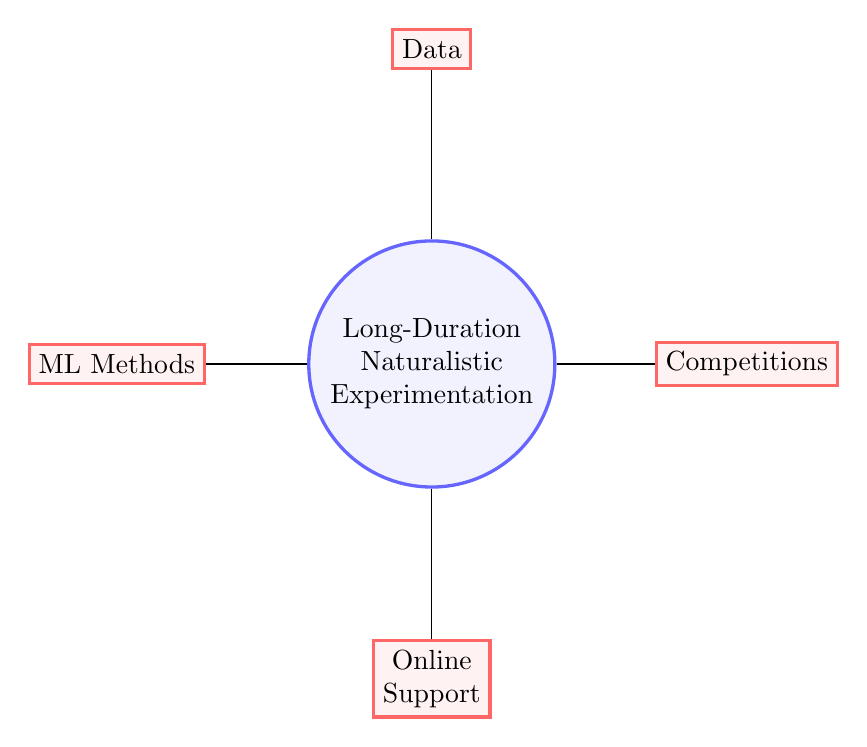
\begin{tikzpicture}[
        node distance=4cm and 1cm,
        centralNode/.style={circle, draw=blue!60, fill=blue!5, very thick,
        minimum size=7mm, align=center},
        itemNode/.style={rectangle, draw=red!60, fill=red!5, very thick,
        minimum size=5mm, align=center},
    ]
    \node[centralNode] (ldnExp)                                 {Long-Duration\\Naturalistic\\Experimentation};
    \node[itemNode]    (dataRepo)           [above of=ldnExp]   {Data};
    \node[itemNode]    (methodsRepo)        [left of=ldnExp]    {ML Methods};
    \node[itemNode]    (competitionsRepo)   [right of=ldnExp]   {Competitions};
    \node[itemNode]    (onlineSupport)      [below of=ldnExp]   {Online\\Support};
    \draw[-] (ldnExp) -- (dataRepo);
    \draw[-] (ldnExp) -- (methodsRepo);
    \draw[-] (ldnExp) -- (competitionsRepo);
    \draw[-] (ldnExp) -- (onlineSupport);
\end{tikzpicture}

    \end{center}
    \caption{Resource theme (blue) and deliverables (red).}
    \label{fig:resource}
\end{figure}

Data generated by our long-duration and naturalistic foraging experiments will
be made publicly available, following FAIR standards, in the
\href{https://dandiarchive.org/}{DANDI} archive.

Whenever possible we will distribute offline and online implementations of all
data analysis methods.
%
Funded by a BBR
award\footnote{\url{https://gow.bbsrc.ukri.org/grants/AwardDetails.aspx?FundingReference=BB\%2FW019132\%2F1}}
we at the SWC, GCNU and NeuroGEARS are adding machine learning methods to
Bonsai. This project will use will use these methods, add a few more methods to
Bonsai, and use them to intelligently control our long-duration naturalistic
foraging experiments with Bonsai.

We will initially distribute methods that we have already used for our foraging
experiments. For several functionalities we have used more than one method, and
we will distribute all of them. In this way experimental neuroscientists using
our resource should be able to compare different distributed methods and choose
the one more suitable to their needs.

The capability to simulate realistic foraging behaviour is important for our
experiments. First, we often have to decide between several options to
configure our foraging arenas (e.g., should we use two or three foraging
patches? how much distance should mice travel to obtain a pellet? where should
patches be located?). It would be helpful to evaluate the different options on
simulated experiments, rather than evaluating them on expensive real
ones. Second, we are often interested in understanding how much the
behaviour of mice in our experiments differ from optimal behaviour. To address
this issue we will simulate foraging agents and
compare their behaviours with those of real mice.

We will encourage contributions from machine learning method developers
interested in applying their methods to data generated by our foraging
experiments. To motivate them to contribute their methods we will organise data
competitions where participants will be given a data problem to solve (e.g., to
simulate a given environment or to analyse a given dataset), they will provide
their solutions, and we will select the winning one.

\subsubsection*{Intelligent experimental control with Bonsai}

Bonsai is a reactive visual programming environment developed by NeuroGEARS Ltd
that is widely used in Neuroscience for controlling sophisticated neuroscience
experiments. Reactive programs are very different from procedural ones (like C
or Python). The main entity of a reactive program is stream and a reactive
program is a sequence of stream transformations that get an input stream,
transform it, and generate an output one. Reactive programs are ideal to
process online data, like those generated in animal neuroscience experiments.

Not all algorithms that we propose to distribute in this resource admit and
online implementation, however most of them do. Whenever possible, we will
distribute online versions implemented in Bonsai of the methods in this
resource.

Online machine learning methods are relevant to long-duration naturalistic
experimentation for at least two reasons. First the extremely large size of
recorded dataset may forbid storing all raw data and online machine learning
algorithms can help decide what data to store. For instance, we want to record
the behaviour of multiple animals in large arenas with high resolution. This
requires using multiple high-definition cameras to record videos of different
parts of the arena. It is not feasible to store the videos by all cameras in
long duration experiments. To overcome this problem, we can use probabilistic
machine learning methods to track online the positions of the mice in the
arena. When the tracking confidence of this methods is high, we would only save
the high-resolution videos of the cameras filming mice, but when their
confidence is low we would save the videos of all cameras.

Second, we want to make neural interventions informed by online inferences from
machine learning methods. For example, in a foraging experiment we could find
that a neural latent variable peaks before the instant when a mouse start
accelerating to leave the current patch (the latent variable could be estimated
using a Poisson linear dynamical system and the acceleration using a linear
dynamical
system\footnote{\url{https://github.com/joacorapela/lds_python/blob/master/docs/tracking/tracking.pdf}}).
We could hypothesise that the neural population associated with the latent
variable is responsible for the decision of leaving a patch. We could then test
this hypothesis by optogenetically silencing this population while an animal is
on a patch and checking if it leaves the patch or not.

\subsubsection*{Resource background}

In July 2020 the SWC began building hardware and software infrastructure to
record behaviour and neural activity of freely moving mice foraging in large
arenas. Our initial focus was on monitoring behaviour for extended periods of
time. We have been able to record behavioral videos, monitor the movement of
the foraging wheels, register pellet deliveries and record mice weight for up
to two weeks in experiments with two mice.
%
More recently we have been able to record behaviour (as described above) and
neural activity (Neuropixel array, four shanks, 384 electrodes per shank)
continuously for up to 27 hours.
%
Our next target is to record behavioral and electrophysiology data continuously
for one month.

We expect that a position paper describing our foraging experiments will be
published by the end of 2024.

\subsubsection*{Why is the proposed resource unique and timely}

% why is the resource unique and timely

Long-duration and naturalistic experimentation is the future of experimental
neuroscience.  Animal foraging is a central neuroscience problem today and
multiple groups around the world are working on it (e.g., Allen Institute for
Neural Dynamics, Janelia Farm, University of Konstanz). Yet, none of this
groups is focused on the unique long-duration and naturalistic experiments that
we are developing at the SWC.
%
The foraging data and the machine learning methods that we propose to
distribute are key elements for world-class foraging research.
%
If this resource is not created the emergence of naturalistic experimentation
will be delayed and the UK may miss the opportunity of becoming a world leader
on this new type of experimentation.

The US Brain Research through Advancing Innovative Neurotechnologies (BRAIN)
initiative~\citep{jorgensonEtAl15} funded projects focused on data analysis
with advanced machine learning methods for long-duration and complex experiment
that we propose to address in this project. However, no BRAIN initiative
project generated the unique long-duration and naturalistic neuroscience
experimental data that we are creating at the SWC.

We have focused this proposal on applications of naturalistic and long-duration
experimentation to experimental neuroscience. However, this type of
experimentation is relevant to other scientific disciplines. For example, it
could we useful to improve the health of plants. We could perform long-duration
experiments on the wild measuring many quantities from the plant environment
(e.g., water, light, temperature, mineral nutrients, humidity) and from the
plant physiology (e.g., photosynthesis, bud burst). We could then study how the
environment affects plant physiology and health across multiple scales. Close
loop interventions could then be performed (e.g., increasing water delivery) to
improve the plant health.

\subsubsection*{Why are we a suitable team to create this resource?}

We (the SWC, GCNU and NeuroGEARS) are an excellent team to develop the proposed
resource. The SWC is at the forefront of experimental neuroscience research and
has been developing mice foraging experiments for five years. The GCNU is a
leader in computational neuroscience and machine learning, with ample
experience in building methods to characterise neural data, and more recently
in distributing openly machine learning methods. And NeuroGEARS has more than a
decade of experience building high-quality software for experimental
neuroscience. We collaborate extensively in a wide range of projects.



\pagebreak

\subsection{Approach}

{\color{red}
Word limit: 4,400

How are you going to deliver your proposed work?

What the assessors are looking for in your response

Explain how you have designed your approach so that it:

\begin{itemize}
	\item is effective and appropriate to achieve your objectives

	\item is feasible, and comprehensively identifies any risks to delivery and how they
will be managed

	\item uses a clearly written and transparent methodology (if applicable)

	\item summarises the previous work and describes how this will be built upon and
progressed (if applicable)

	\item will maximise translation of outputs into outcomes and impacts

	\item describes how your, and if applicable your team’s, research environment (in
terms of the place and relevance to the project) will contribute to the success
of the work

\end{itemize}

Include the following when describing your approach:

\begin{itemize}

	\item measurable targets against which the outcome of the work will be assessed

	\item significant technical details for the development, maintenance or
enhancement of the resource, indicating how this is of internationally
exceptional quality

	\item any proposed research efforts and how they directly facilitate development of
the resource (if applicable)

	\item if the focus is on maintaining an existing resource instead of suggesting
further development, provide evidence of why significant upgrades are not
required at this time and detail why the resource needs continued support to
maintain world-leading functionality (if applicable)

\end{itemize}

Describe the specific contribution of each applicant to the proposed resource:

\begin{itemize}

	\item their scientific contributions, for example, research field and specialist
knowledge, experience, resource management expertise, technical and data
analysis expertise

	\item their role and responsibilities, for example, managerial, leadership, mentoring
	\item references to specific work packages are recommended
	\item highlight where applicants will work collaboratively to deliver specific project
requirements
	\item include clear time commitments for each applicant
\end{itemize}

There is no need to duplicate information included in the ‘Applicant and team
capability to deliver’ section.

References may be included within this section.

You may demonstrate elements of your responses in visual form if relevant.
Further details are provided in the Funding Service.

A project Gannt chart is compulsory and should be inserted as an image at the
very end of this section. The Gannt chart should identify appropriate
deliverables, responsibilities and time points for each objective.
}

The proposed resource will distribute machine learning methods to process
behavioural data and neural data, to perform simulations and to do data
compression. The resource will also distribute data from our foraging
experiments that will be used to demonstrate the functionality of all
distributed methods and all method contributed by methods developers.

\subsubsection{Methods to process behavioral measurements}

\paragraph{Linear dynamical systems models}

\paragraph{Nonlinear dynamical systems models}

\paragraph{Hidden Markov models}

\paragraph{Linear regression models}

\paragraph{Deep neural networks}

\paragraph{Switching linear dynamical systems models}

\paragraph{Pose estimation methods}


\subsubsection{Methods to process neural measurements}

\subsubsection{Methods to simulate foraging data}

\subsubsection{Methods for compressing behavioral and neural measurements}



\pagebreak

\subsection{Community demand: letters (or emails) of support}

{\color{red}

Letters (or emails) of support demonstrating community demand are mandatory
for BBR.

Upload a single PDF of maximum 8MB containing a maximum of 10 letters or
emails of support. These should be uploaded in English or Welsh only. Enter
the words ‘attachment supplied’ in the text box.

What the assessors are looking for in your response

The letters should give an indication of community demand for the resource in
question, demonstrating the breadth of research and the high-quality science
relevant to BBSRC remit that the resource would underpin.

Add the following details for each letter:

\begin{enumerate}

	\item the organisation name (searchable via a drop-down list or enter the
organisation’s details manually, as applicable)

	\item contact name of the signatory

\end{enumerate}

Letters of support aimed at demonstrating community demand should:

\begin{enumerate}

	\item outline the uniqueness and expected added value of the proposed resource
to the UK bioscience research community and infrastructure landscape

	\item clearly explain the impact and benefit of the proposed resource on the
writer’s research and the associated community

	\item if possible, explain where this supported research has already demonstrated
or could have potential for particular scientific, economic or societal impact

	\item help to demonstrate the breadth of the relevant user community

\end{enumerate}

Letters of support that fail to do so, in particular template letters indicating
generic support without identifying a particular usage, are of negligible value for
the assessment and should not be submitted. Carefully chosen letters
containing relevant evidence of the requirement or benefit to be gained, are of
greater value than large numbers of letters.

The Funding Service will provide document upload details when you apply.
}

\pagebreak

\subsection{Applicant and team capability to deliver}

{\color{red}

Word limit: 1,650

Why are you the right individual or team to successfully deliver the proposed
work?

What the assessors are looking for in your response

Evidence of how you, and if relevant your team, have:

\begin{itemize}

	\item the relevant experience (appropriate to career stage) to deliver the proposed
work

	\item the right balance of skills and expertise to cover the proposed work

	\item the appropriate leadership and management skills to deliver the work and
your approach to develop others

	\item contributed to developing a positive research environment and wider
community

\end{itemize}

You may demonstrate elements of your responses in visual form if relevant.
Further details are provided in the Funding Service.

The word count for this section is 1,650 words: 1,150 words to be used for R4RI
modules (including references) and, if necessary, a further 500 words for
Additions.

Use the Résumé for Research and Innovation (R4RI) format to showcase the
range of relevant skills you and, if relevant, your team (project and project co-
leads, researchers, technicians, specialists, partners and so on) have and how
this will help deliver the proposed work. You can include individuals’ specific
achievements but only choose past contributions that best evidence their ability
to deliver this work.

Complete this section using the R4RI module headings listed. Use each
heading once and include a response for the whole team, see the UKRI
guidance on R4RI. You should consider how to balance your answer, and
emphasise where appropriate the key skills each team member brings:

\begin{itemize}

	\item contributions to the generation of new ideas, tools, methodologies,
or knowledge

	\item the development of others and maintenance of effective working relationships

	\item contributions to the wider research and innovation community

	\item contributions to broader research or innovation users and audiences
and towards wider societal benefit

\end{itemize}

Additions

Provide any further details relevant to your application. This section is optional
and can be up to 500 words. You should not use it to describe additional skills,
experiences, or outputs, but you can use it to describe any factors that provide
context for the rest of your R4RI (for example, details of career breaks if you
wish to disclose them).

Complete this as a narrative. Do not format it like a CV.

There is no need to duplicate information included in the ‘Approach’ section.

UKRI has introduced new role types for funding opportunities being run on the
new Funding Service.

For full details, see \href{https://www.ukri.org/apply-for-funding/before-you-apply/check-if-you-are-eligible-for-research-and-innovation-funding/eligibility-as-an-individual/#contents-list}{Eligibility as an individual}.

References may be included within this section.

}

\pagebreak

\subsection{Project partners}

{\color{red}

Add details about any project partners’ contributions. If there are no project
partners, you can indicate this on the Funding Service.

A project partner is a collaborating organisation who will have an integral role in
the proposed research. This may include direct (cash) or indirect (in-kind)
contributions such as expertise, staff time or use of facilities.

Add the following project partner details:

\begin{itemize}

	\item the organisation name and address (searchable via a drop-down list or enter
the organisation’s details manually, as applicable)

	\item the project partner contact name and email address

	\item the type of contribution (direct or in-direct) and its monetary value

\end{itemize}

If a detail is entered incorrectly and you have saved the entry, remove the
specific project partner record and re-add it with the correct information.

For audit purposes, UKRI requires formal collaboration agreements to be put in
place if an award is made.

}

\pagebreak

\subsection{Project partners: letters (or emails) of support}

{\color{red}

Upload a single PDF containing the letters or emails of support from each
partner you named in the Project Partner section. These should be uploaded in
English or Welsh only.

Enter the words ‘attachment supplied’ in the text box, or if you do not have any
project partners enter N/A.

What the assessors are looking for in your response
Each letter or email you provide should:

\begin{itemize}

	\item confirm the partner’s commitment to the project

	\item clearly explain the value, relevance, and possible benefits of the work to
them

	\item describe any additional value that they bring to the project

\end{itemize}

The Funding Service will provide document upload details when you apply. If
you do not have any project partners, you will be able to indicate this in the
Funding Service.

Ensure you have prior agreement from project partners so that, if you are
offered funding, they will support your project as indicated in the project
partners’ section.

For audit purposes, UKRI requires formal collaboration agreements to be put in
place if an award is made.

}

\pagebreak

\subsection{Management strategy}

{\color{red}

Word limit: 500

How do you plan to manage the resource?

What the assessors are looking for in your response

\begin{enumerate}

	\item resources will be expected to have governance arrangements appropriate for
the oversight and successful delivery of the project’s complexity
	\item provide details about the project’s management and advisory structure
	\item provide details of the approach to project and risk management, and the
monitoring strategy for tracking progress of the proposed programme
	\item provide details on how demand and access requests will be managed, and
what support will be provided to the users of the resource
	\item an advisory board is required for all projects, which is independent from both
the academic institutions and project partners involved in the proposal.
Provide information on the proposed membership of this advisory board and
how it will be used
	\item provide details on how the resource user perspective and their needs will be
considered, including how feedback will be sought and subsequently used to
inform the management of the resource

\end{enumerate}

You may demonstrate elements of your responses in visual form if relevant.
Further details are provided in the Funding Service.
}

\pagebreak

\subsection{Data management and sharing}

{\color{red}

Word limit: 1,500

How will you manage and share data collected or acquired as part of the
proposed resource?

What the assessors are looking for in your response

Provide a data management plan using the \href{https://www.ukri.org/wp-content/uploads/2024/03/BBSRC-110324-Funding-Opp-BioinformaticsBiologicalResourcesFund-DataManagementPlanTemplate.pdf}{BBR DMP template (PDF, 161KB)}
structure that clearly details how your proposed resource will comply with
UKRI’s published \href{https://www.ukri.org/manage-your-award/publishing-your-research-findings/making-your-research-data-open/} data sharing policy, which includes detailed guidance notes.

}

\pagebreak

\subsection{Trusted Research and Innovation (TR\&I)}

{\color{red}

Word limit: 500

Does the proposed work involve international collaboration in a sensitive
research or technology area?

What the assessors are looking for in your response

Demonstrate how your proposed international collaboration relates to trusted
research and innovation, including:

\begin{itemize}

	\item list the countries your international project co-leads, project partners and
visiting researchers, or other collaborators are based in

	\item if international collaboration is involved, explain whether this project is
relevant to one or more of the \href{https://www.gov.uk/government/publications/national-security-and-investment-act-guidance-on-notifiable-acquisitions/national-security-and-investment-act-guidance-on-notifiable-acquisitions}{17 areas} of the UK National Security and
Investment (NSI) Act

	\item if one or more of the \href{https://www.gov.uk/government/publications/national-security-and-investment-act-guidance-on-notifiable-acquisitions/national-security-and-investment-act-guidance-on-notifiable-acquisitions}{17 areas} of the UK National Security and Investment
(NSI) Act are involved, please identify which areas

\end{itemize}

If your proposed work does not involve any international collaboration, answer
‘n/a’ here.

We may ask you to provide additional information about how your proposed
project will comply with our approach and expectation towards TR\&I, identifying
potential risks and the relevant controls you will put in place to help
proportionately reduce these risks.

}

\pagebreak

\subsection{Resources and cost justification}

{\color{red}

Word limit: 1,000

What will you need to deliver your proposed work and how much will it cost?

What the assessors are looking for in your response

Justify the application’s more costly resources, in particular:

\begin{itemize}

	\item project staff

	\item significant travel for field work or collaboration (but not regular travel between collaborating organisations or to conferences)

	\item any equipment that will cost more than £10,000

	\item any consumables beyond typical requirements, or that are required in exceptional quantities

	\item all facilities and infrastructure costs

	\item all resources that have been costed as ‘Exceptions’

\end{itemize}

Assessors are not looking for detailed costs or a line-by-line breakdown of all project resources. Overall, they want you to demonstrate how the resources you anticipate needing for your proposed work:

are comprehensive, appropriate, and justified
\begin{itemize}

	\item represent the optimal use of resources to achieve the intended outcomes

	\item maximise potential outcomes and impacts

	\item evidence appropriate consideration for alternative long-term sustainability options beyond BBSRC funding

\end{itemize}

}

\pagebreak

\subsection{Your organisation’s support}

{\color{red}

Word limit: 500

Provide details of support from your research organisation and project co-lead research organisations.

What the assessors are looking for in your response

Provide a statement of support from all participating research organisations
detailing why they are best placed to support the proposed project. This should
include details of any matched funding that will be provided to support the
activity and any additional support that might add value to the work.

Assessors will be looking for a strong statement of commitment from your research organisations.

BBSRC recognises that in some instances, this information may be provided by the Research Office, the Technology Transfer Office (TTO) or equivalent, or a combination of both.

You must also include the following details:

\begin{itemize}

	\item a significant person’s name and their position, from the TTO or
Research Office, or both

	\item office address or web link

\end{itemize}

Upload details are provided within the service on the actual application.

We do not require separate institutional letters of support as attachments. By
submitting your application to us, you are confirming that your institutions
are supportive of and committed to your project.

}

\bibliographystyle{apalike}
\bibliography{linearDynamicalSystems,stateSpaceModels,machineLearning,epilepsy,latentsVariablesModels,deepNeuralNets,monitoringBehavior,dataSharing,misc,others}
\end{document}
